%%%%%%%%%%%%%%%%%%%%%%%%%%%%%%%%%%%%%%%%%%%%%%%%%%%%%%%%%%%%%%%%%%%%%%%%%%%%%%%%%%%%%%%
%%%  What's up LOD Cloud - Observing The State of Linked Open Data Cloud Metadata  %%%%
%%%%%%%%%%%%%%%%%%%%%%%%%%%%%%%%%%%%%%%%%%%%%%%%%%%%%%%%%%%%%%%%%%%%%%%%%%%%%%%%%%%%%%%

\documentclass[runningheads,a4paper]{llncs}

\usepackage[utf8]{inputenc}
\usepackage{amssymb}
\setcounter{tocdepth}{3}
\usepackage{graphicx}
\usepackage{tabularx}
\usepackage{url}
\usepackage{listings}
\usepackage{subfigure}
\usepackage{algorithmic}
\usepackage{algorithm}
\usepackage{xcolor}
\usepackage{caption}
\usepackage{multirow}
\usepackage[T1]{fontenc}

\graphicspath{ {figures/} }

\newcommand{\keywords}[1]{\par\addvspace\baselineskip
\noindent\keywordname\enspace\ignorespaces#1}

% todo macro
\usepackage{color}
\newtheorem{deflda}{Axiom}
\newcommand{\todo}[1]{\noindent\textcolor{red}{{\bf \{TODO}: #1{\bf \}}}}

\colorlet{punct}{red!60!black}
\definecolor{background}{HTML}{FFFFFF}
\definecolor{delim}{RGB}{20,105,176}

% Language Definitions for JSON
\lstdefinelanguage{json}{
		basicstyle=\tiny,
    numbersep=4pt,
    showstringspaces=false,
    breaklines=true,
    frame=lines,
    literate=
      {:}{{{\color{punct}{:}}}}{1}
      {,}{{{\color{punct}{,}}}}{1}
      {[}{{{\color{delim}{[}}}}{1}
      {]}{{{\color{delim}{]}}}}{1},
}

%%%%%%%%%%%%%%%%%%%%%%%%%%%%%%%
%%%  Beginning of document  %%%
%%%%%%%%%%%%%%%%%%%%%%%%%%%%%%%

\begin{document}

% first the title is needed
\title{What's up LOD Cloud?}
\subtitle{Observing The State of\\Linked Open Data Cloud Metadata}

\author{Ahmad Assaf\inst{1}\inst{2}, Aline Senart\inst{2} and Rapha\"{e}l Troncy\inst{1} }

\institute{EURECOM, Sophia Antipolis, France, \email{<firstName.lastName@eurecom.fr>}
  \and SAP Labs France, \email{<firstName.lastName@sap.com>}
}

% a short form should be given in case it is too long for the running head
\titlerunning{Observing The State of Linked Open Data Cloud Metadata}
%\authorrunning{Assaf, Senart and Troncy}

\maketitle

%%%%%%%%%%%%%%%%%%
%%%  Abstract  %%%
%%%%%%%%%%%%%%%%%%

\begin{abstract}
Linked Open Data (LOD) has emerged as one of the largest collections of interlinked datasets on the web. In order to benefit from this mine of data, one needs to access descriptive information about each dataset (or metadata). However, the heterogeneous nature of data sources reflects directly on the data quality as these sources often contain inconsistent as well as misinterpreted and incomplete metadata information. Considering the significant variation in size, the languages used and the freshness of the data, one realizes that finding useful datasets without prior knowledge is increasingly complicated. We have developed Roomba, a tool that enables to validate, correct and generate dataset metadata. In this paper, we present the results of running this tool on parts of the LOD cloud accessible via the datahub.io API. The results demonstrate that the general state of the datasets needs more attention as most of them suffers from bad quality metadata and lacking some informative metrics that are needed to facilitate dataset search. We also show that the automatic corrections done by Roomba increase the overall quality of the datasets metadata and we highlight the need for manual efforts to correct some important missing information.

\keywords{Dataset Profile, Metadata, Data Quality, Data Portal}
\end{abstract}

%%%%%%%%%%%%%%%%%%%%%%%%%
%%%  1. Introduction  %%%
%%%%%%%%%%%%%%%%%%%%%%%%%

\section{Introduction}
\label{sec:introduction}
The Linked Open Data (LOD) cloud\footnote{The datahub.io view of the LOD cloud is at \url{http://datahub.io/dataset?tags=lod}} has grown significantly in the past years, offering various datasets covering a broad set of domains from life sciences to media and government data~\cite{BizerHeath2009}. To maintain high quality data, publishers should comply with a set of best practices detailed in~\cite{Bizer:2011:EWG:2075914.2075915}. Metadata provisioning is one of those best practices requiring publishers to attach metadata needed to effectively understand and use datasets.

Data portals expose metadata via various models. A model should contain the minimum amount of information that conveys to the inquirer the nature and content of its resources~\cite{nebert2004developing}. It should contain information to enable data discovery, exploration and exploitation. We divided the metadata information into the following:
\begin{itemize}
 \item \textbf{General information}: General information about the dataset (e.g. title, description, ID). This general information is manually filled by the dataset owner. In addition to that, tags and group information is required for classification and enhancing dataset discoverability.
 \item \textbf{Access information}: Information about accessing and using the dataset. This includes the dataset URL, some license information (i.e. license title and URL) and information about the datasets resources. Each resource has generally a set of attached metadata (e.g. resource name, URL, format, size).
 \item \textbf{Ownership information}: Information about the ownership of the dataset (e.g. organization details, maintainer details, author). The existence of this information is important to identify the authority on which the generated report and the newly corrected profile will be sent to.
 \item \textbf{Provenance information}: Temporal and historical information on the dataset and its resources (e.g. creation and update dates, version information, version number). Most of this information can be automatically filled and tracked.
\end{itemize}

Data portals are datasets' access points providing tools to facilitate data publishing, sharing, searching and visualization. CKAN\footnote{\url{http://ckan.org}} is the world's leading open-source data portal platform powering web sites like the Datahub which hosts the LOD cloud metadata. We have created Roomba~\cite{Assaf:WWW15}, a tool that automatically validates, corrects and generates dataset metadata. Since we are evaluating the LOD cloud metadata, we validate the datasets against the CKAN standard model\footnote{\url{http://demo.ckan.org/api/3/action/package_show?id=adur_district_spending}}. The results demonstrate that the general state of the examined datasets needs much more attention as most of the datasets suffers from bad quality metadata and lacking some informative metrics needed that would facilitate dataset search. The noisiest metadata values were access information such as licensing information and resource descriptions in addition to large numbers of resource reachability problems. We also show that the automatic corrections of the tool increase the overall quality of the datasets metadata and highlight the need for manual efforts to correct some important missing information.

%%%%%%%%%%%%%%%%%%%%%%%%%
%%%  2. Related Work  %%%
%%%%%%%%%%%%%%%%%%%%%%%%%

\section{Related Work}
\label{sec:related-work}
The Data Catalog Vocabulary (DCAT)~\cite{Erickson:14:DCV} and the Vocabulary of Interlinked Datasets (VoID)~\cite{Cyganiak:11:DLD} are models for representing RDF datasets metadata. There exist several tools aiming at exposing dataset metadata using these vocabularies such as \cite{BoHm:2011:CVD:2030805.2031001}.
Few approaches tackle the issue of examining datasets metadata. The Project Open Data Dashboard\footnote{\url{http://labs.data.gov/dashboard/}} validator analyzes machine readable files for automated metrics to check their alignment with the Open Data principles. Similarly on the LOD cloud, the Datahub LOD Validator\footnote{\url{http://validator.lod-cloud.net/}} checks a dataset compliance for inclusion in the LOD cloud. However, it lacks the ability to give detailed insights about the completeness of the metadata and an overview on the state of the entire LOD cloud group.

The \textit{State of the LOD Cloud Report}~\cite{SOLOD} measures the adoption of Linked Data best practices back in 2011. More recently, the authors in~\cite{DBLP:conf/semweb/SchmachtenbergBP14} used LDSpider~\cite{conf/semweb/IseleUBH10} to crawl and analyze 1014 different datasets in the web of Linked Data in 2014. While these reports expose important information about datasets like provenance, licensing and accessibility, they do not cover the entire spectrum of metadata categories as presented in~\cite{Framework2012}.

%%%%%%%%%%%%%%%%%%%%%%%%%%%%%%%%%%%%%%%
%%%  3. Experiments and Evaluation  %%%
%%%%%%%%%%%%%%%%%%%%%%%%%%%%%%%%%%%%%%%

\section{Experiments and Evaluation}
\label{sec:experiment}
In this section, we describe our experiments when running the Roomba tool on the LOD cloud. All the experiments are reproducible by our tool and their results are available on its Github repository at \url{https://github.com/ahmadassaf/opendata-checker}.

\subsection{Experimental Setup}
The current state of the LOD cloud report~\cite{DBLP:conf/semweb/SchmachtenbergBP14} indicates that there are more than 1014 datasets available. These datasets have been harvested by the LDSpider crawler~\cite{conf/semweb/IseleUBH10} seeded with 560 thousands URIs. However, since Roomba requires the datasets metadata to be hosted in a data portal where either the dataset publisher or the portal administrator can attach relevant metadata to it, we rely on the information provided by the Datahub CKAN API. We consider two possible groups: the first one tagged with ``lodcloud'' returns 259 datasets, while the second one tagged with ``lod'' returns only 75 datasets. We manually inspect these two lists and find out that the API result for the tag ``lodcloud'' is the correct one. The 259 datasets contain a total of 1068 resources. We run the instance and resource extractor from Roomba in order to cache the metadata files for these datasets locally and we launch the validation process which takes around two and a half hours on a 2.6 Ghz Intel Core i7 processor with 16GB of DDR3 memory machine.

\subsection{Results and Evaluation}
CKAN dataset metadata includes three main sections in addition to the core dataset's properties. Those are the \textbf{groups}, \textbf{tags} and \textbf{resources}. Each section contains a set of metadata corresponding to one or more metadata type. For example, a dataset resource will have general information such as the resource name, access information such as the resource url and provenance information such as creation date. The framework generates a report aggregating all the problems in all these sections, fixing field values when possible. Errors can be the result of missing metadata fields, undefined field values or field value errors (e.g. unreachable URL or incorrect email address).

Figures \ref{fig:metadata_noise_by_metadata_type} and \ref{fig:metadata_noise_by_metadata_type} show the percentage of errors found in metadata fields by section and by information type respectively. We observe that the most erroneous information for the dataset core information is related to ownership since this information is missing or undefined for 41\% of the datasets. Datasets resources have the poorest metadata. 64\% of the general metadata, all the access information and 80\% of the provenance information contain missing or undefined values. Table \ref{tab:top_metadata_fields_errors} shows the top metadata fields errors for each metadata information type.

\begin{table}
\begin{center}
\begin{tabular}{|c|c|c|c|c|c|}
\hline
\multicolumn{2}{|c|}{Metadata Field} & Error \% & Section & Error Type & Auto Fix\tabularnewline
\hline
\hline
\multirow{6}{*}{General } & group & 100\% & Dataset & Missing & -\tabularnewline
\cline{2-6}
 & vocabulary\_id & 100\% & Tag & Undefined & -\tabularnewline
\cline{2-6}
 & url-type & 96.82\% & Resource & Missing & -\tabularnewline
\cline{2-6}
 & mimetype\_inner & 95.88\% & Resource & Undefined & Yes\tabularnewline
\cline{2-6}
 & hash & 95.51\% & Resource & Undefined & Yes\tabularnewline
\cline{2-6}
 & size & 81.55\% & Resource & Undefined & Yes\tabularnewline
\hline
\multirow{5}{*}{Access } & cahce\_url & 96.9\% & Resource & Undefined & -\tabularnewline
\cline{2-6}
 & webstore\_url & 91.29\% & Resource & Undefined & -\tabularnewline
\cline{2-6}
 & license\_url & 54.44\% & Dataset & Missing & Yes\tabularnewline
\cline{2-6}
 & url & 30.89\% & Resource & Unreachable & -\tabularnewline
\cline{2-6}
 & license\_title & 16.6\% & Dataset & Undefined & Yes\tabularnewline
\hline
\multirow{5}{*}{Provenance } & cache\_last\_updated & 96.91\% & Resource & Undefined & Yes\tabularnewline
\cline{2-6}
 & webstore\_last\_updated & 95.88\% & Resource & Undefined & Yes\tabularnewline
\cline{2-6}
 & created & 86.8\% & Resource & Missing & Yes\tabularnewline
\cline{2-6}
 & last\_modified & 79.87\% & Resource & Undefined & Yes\tabularnewline
\cline{2-6}
 & version & 60.23\% & Dataset & Undefined & -\tabularnewline
\hline
\multirow{5}{*}{Ownership } & maintainer\_email & 55.21\% & Dataset & Undefined & -\tabularnewline
\cline{2-6}
 & maintainer & 51.35\% & Dataset & Undefined & -\tabularnewline
\cline{2-6}
 & author\_email & 15.06\% & Dataset & Undefined & -\tabularnewline
\cline{2-6}
 & organization\_image\_url & 10.81\% & Dataset & Undefined & -\tabularnewline
\cline{2-6}
 & author & 2.32\% & Dataset & Undefined & -\tabularnewline
\hline
\end{tabular}
\captionof{table}{Top metadata fields error \% by type}
\label{tab:top_metadata_fields_errors}
\end{center}
\end{table}

We notice that 42.85\% of the top metadata problems can be fixed automatically. Among them, 44.44\% of these problems can be fixed by our tool while the others need tools that are plugged into the data portal. We further present and discuss the results grouped by metadata information type in the following sub-sections.

\subsection{General information}
34 datasets (13.13\%) do not have valid \texttt{notes} values. \texttt{tags} information for the datasets are complete except for the \texttt{vocabulary\_id} as this is missing from all the datasets' metadata. All the datasets \texttt{groups} information are missing \texttt{display\_name, description, title, image\_display\_url, id, name}. After manual examination, we observe a clear overlap between group and organization information. Many datasets like \texttt{event-media} use the organization field to show group related information (being in the LOD Cloud) instead of the publishers details.

\subsection{Access information}
25\% of the datasets access information (being the dataset URL and any URL defined in its groups) have issues: generally missing or unreachable URLs. 3 datasets (1.15\%) do not have a URL defined (tip, uniprot\-databases, uniprot\-citations) while 45 datasets (17.3\%) defined URLs are not accessible at the time of writing this paper. One dataset does not have resources information (bio2rdf\-chebi) while the other datasets have a total of 1068 defined resources.

On the datasets resources level, we notice wrong or inconsistent values in the \texttt{size} and \texttt{mimetype} fields. However, 44 datasets have valid \texttt{size} field values and 54 have valid \texttt{mimetype} field values but they were not reachable, thus providing incorrect information. 15 fields (68\%) of all the other access metadata are missing or have undefined values. Looking closely, we notice that most of these problems can be easily fixed automatically by tools that can be plugged to the data portal. For example, the top six missing fields are the \texttt{cache\_last\_updated}, \texttt{cache\_url}, \texttt{url\-type}, \texttt{webstore\_last\_updated}, \texttt{mimetype\-\_inner} and \texttt{hash} which can be computed and filled automatically. However, the most important missing information which require manual entry are the dataset's \texttt{name} and \texttt{description} which are missing from 817 (76.49\%) and 98 (9.17\%) resources respectively. A total of 334 resources (31.27\%) URLs were not reachable, thus affecting highly the availability of these datasets. CKAN resources can be of various predefined types $(file, file.upload, api, visualization, code and documentation)$. Roomba also breaks down these unreachable resources according to their types: 211 (63.17\%) resources do not have valid \texttt{resource\_type}, 112 (33.53\%) are files, 8 (2.39\%) a re metadata and one (0.029\%) are example and documentation types.

To have more details about the resources URL types, we created a $key:object meta-field values$ group level report on the LOD cloud with \texttt{resources>\\format:title}. This will aggregate the resources format information for each dataset. We observe that only 161 (62.16\%) of the datasets valid URLs have SPARQL endpoints defined using the \texttt{api/sparql} resource format. 92.27\% provided RDF example links and 56.3\% provided direct links to RDF down-loadable dumps.

The noisiest part of the access metadata is about license information. A total of 43 datasets (16.6\%) does not have a defined \texttt{license\_title} and \texttt{license\_id} fields, where 141 (54.44\%) have missing \texttt{license\_url} field.

\begin{figure}
\parbox{7cm}{\hspace*{-.2in}
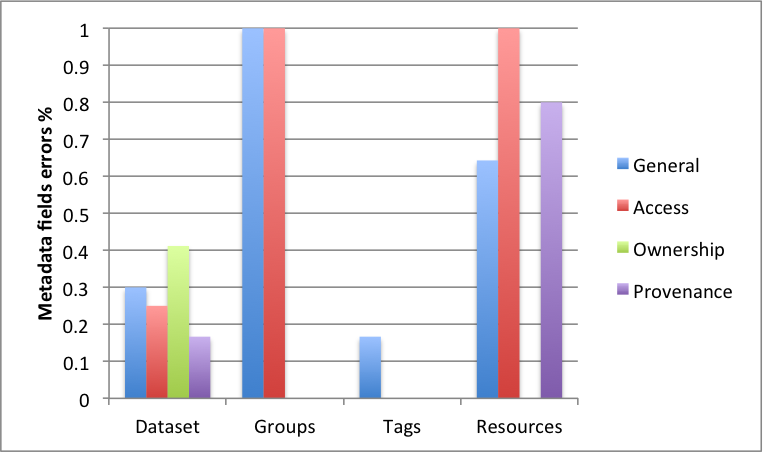
\includegraphics[width=.95\linewidth]{metadata_noise_by_section.png}
\captionsetup{textfont=small,singlelinecheck=off,justification=centering}
\caption{Error \% by section}
\label{fig:metadata_noise_by_section}}
\qquad
\begin{minipage}{7cm}\hspace*{-.6in}
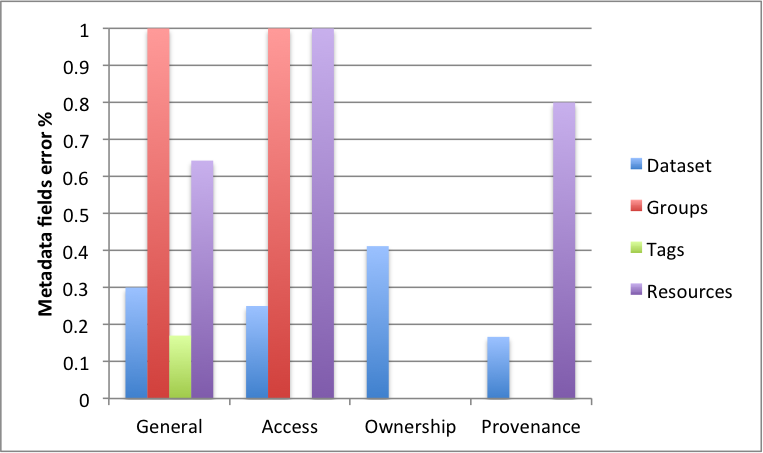
\includegraphics[width=.95\linewidth]{metadata_noise_by_metadata_type.png}
\captionsetup{textfont=small,singlelinecheck=off,justification=raggedright}
\caption{Error \% by information type}
\label{fig:metadata_noise_by_metadata_type}
\end{minipage}
\end{figure}

\subsection{Ownership information}
Ownership information is divided into direct ownership (author and maintainer) and organization information. Four fields (66.66\%) of the direct ownership information are missing or undefined. The breakdown for the missing information is: 55.21\% \texttt{maintainer\_email}, 51.35\% \texttt{maintainer}, 15.06\% \texttt{author\_email}, 2.32\% \texttt{author}. Moreover, our framework performs checks to validate existing email values. 11 (0.05\%) and 6 (0.05\%) of the defined \texttt{author\_email} and \texttt{maintainer\_email} fields are not valid email addresses respectively. For the organization information, two field values (16.6\%) were missing or undefined. 1.16\% of the \\\texttt{organization\_description} and 10.81\% of the \texttt{organization\-\_image\_url} information with two out of these URLs are unreachable.

\subsection{Provenance information}
80\% of the resources provenance information are missing or undefined. However, most of the provenance information (e.g. \texttt{metadata\_created, metadata\_modified}) can be computed automatically by tools plugged into the data portal. The only field requiring manual entry is the \texttt{version} field which was found to be missing in 60.23\% of the datasets.

\subsection{Enriched Profiles}
Roomba can automatically fix, when possible, the license information (title, url and id) as well as the resources mimetype and size.

20 resources (1.87\%) have incorrect \texttt{mimetype} defined, while 52 resources (4.82\%) have incorrect \texttt{size} values. These values have been automatically fixed based on the values defined in the HTTP response header.

We have noticed that most of the issues surrounding license information are related to ambiguous entries. To resolve that, we manually created a mapping file\footnote{\url{https://github.com/ahmadassaf/opendata-checker/blob/master/util/licenseMappings.json}} standardizing the set of possible license names and urls using the open source and knowledge license information\footnote{\url{https://github.com/okfn/licenses}}. As a result, we managed to normalize 123 (47.49\%) of the datasets' license information.

To check the impact of the corrected fields, we seeded Roomba with the enriched profiles. Since Roomba uses file based cache system, we simply replaced all the datasets \texttt{json} files in the \texttt{\textbackslash cache\textbackslash datahub.io\textbackslash datasets} folder with those generated in \texttt{\textbackslash cache\textbackslash datahub.io\textbackslash enriched}. After running Roomba again on the enriched profiles, we observe that the errors percentage for missing \texttt{size} fields decreased by 32.02\% and for \texttt{mimetype} fields by 50.93\%. We also notice that the error percentage for missing \texttt{license\_urls} decreased by 2.32\%.

%%%%%%%%%%%%%%%%%%%%%%%%%%%%%%%%%%%%%%%%%
%%%  4. Conclusion and Future Work  %%%%%
%%%%%%%%%%%%%%%%%%%%%%%%%%%%%%%%%%%%%%%%%

\section{Conclusion and Future Work}
\label{sec:conclusion}
In this paper, we presented the results of running Roomba over the LOD cloud group hosted in the Datahub. We discovered that the general state of the examined datasets needs attention as most of them lack informative access information and their resources suffer low availability. These two metrics are of high importance for enterprises looking to integrate and use external linked data. We found out that the most erroneous information for the dataset core information are ownership related since this information is missing or undefined for 41\% of the datasets. Datasets resources have the poorest metadata: 64\% of the general metadata, all the access information and 80\% of the provenance information contained missing or undefined values.

We also show that the automatic correction process can effectively enhance the quality of some information. We believe there is a need to have a community effort to manually correct missing important information like ownership information (maintainer, author, and maintainer and author emails). As part of our future work, we plan to run Roomba on various data portals and perform a detailed comparison to check the metadata health of LOD datasets against those in other prominent data portals.

%%%%%%%%%%%%%%%%%%%%%%%%%
%%%  Acknowledgments  %%%
%%%%%%%%%%%%%%%%%%%%%%%%%

\section*{Acknowledgments}
This research has been partially funded by the European Union's 7th Framework Programme via the project Apps4EU (GA No. 325090).

\bibliographystyle{abbrv}
\nocite{*}
\bibliography{SUP}
\end{document}
